\documentclass[10pt]{beamer}

% Paquets LaTeX 
\usepackage[french]{babel}
\usepackage[T1]{fontenc}
\usepackage{type1ec}
\usepackage[utf8]{inputenc}
\usepackage{lmodern}            % pour sf et tt
\usepackage{fourier}            % pour rm
\usepackage{textcomp}           % pour \textcopyleft
\usepackage{ccicons}            % pour les Creative Commons
\usepackage{array}              % pour faciliter les styles de tableaux
\newcolumntype{^}{>{\global\let\currentrowstyle\relax}}
\newcolumntype{$}{>{\currentrowstyle}}%$
\newcommand{\rowstyle}[1]{\gdef\currentrowstyle{#1}#1\ignorespaces}
\usepackage{hyperref}

% Paramétrage Beamer & co
\uselanguage{french}
\languagepath{french}
\deftranslation[to=french]{Definition}{Définition}
\usefonttheme[stillsansseriflarge]{serif}
\usefonttheme[onlylarge]{structurebold}
\mode<presentation>
\setbeamercovered{dynamic}
\setbeamertemplate{footline}
{
  \leavevmode%
  \hbox{%
  \begin{beamercolorbox}[wd=\paperwidth,ht=2.25ex,dp=1ex,right]{frametitle}
    \usebeamerfont{date in head/foot}
    \insertframenumber{} / \inserttotalframenumber\hspace*{2ex} 
  \end{beamercolorbox}}%
  \vskip0pt%
}
\setbeamertemplate{sections/subsections in toc}[sections numbered]
\setbeamertemplate{navigation symbols}{}
\setbeamertemplate{blocks}[rounded][shadow=true]
\setbeamertemplate{items}[ball]
\setbeamerfont{block title}{size={}}
\usecolortheme{orchid}
\setbeamersize{text margin left=1em,text margin right=1em}
\mode
<all>
\hypersetup{colorlinks,linkcolor=,urlcolor=blue} % liens en bleu

% Méta-données 
\title[Le logiciel libre]{%
  
\includegraphics[width=.2\columnwidth]{gnu-head}\\
  Le logiciel libre}
\titlegraphic{\includegraphics[width=5em]{logo-lille1}}
\author[B. Beaufils]{Bruno BEAUFILS}
\institute[Lille 1]{\textbf{Université~Lille~1}}
\date{4 février 2014\\{\ccbyncsa}\\\textbf{\scriptsize CC-BY-NC-SA}}
\subject{Logiciel libre}
\keywords{logiciel libre, free software, floss}

%%%%%%%%%%%%%%%%%%%%%%%%%%%%%%%%%%%%%%%%%%%%%%%%%%%%%%%%%%%%%%%%%%%%%%%%%%%%%%

\begin{document}

\maketitle

%%%%%%%%%%%%%%%%%%%%%%%%%%%%%%%%%%%%%%%%%%%%%%%%%%%%%%%%%%%%%%%%%%%%%%%%%%%%%%

\begin{frame}
  \frametitle{Présentation \only<1>{(Jekyll)}\only<2>{(Hide)}}

  \begin{center}
    \Large
    \vfill
    \textbf{Bruno BEAUFILS}
    \vfill
    \only<1>{Maître de conférences en informatique}
    \only<2>{Libriste convaincu depuis 1991}
    \vfill\vfill
    \only<1>{\url{bruno.beaufils@univ-lille1.fr}}
    \only<2>{\url{bruno+libre@boulgour.com}}
    \vfill
    \only<1>{\url{http://www.lifl.fr/~beaufils}}
    \only<2>{\url{http://bruno.boulgour.com}}
    \vfill
    \only<1>{Bureau IUT-4A49 ou M3-222}
    \only<2>{\url{@brunobeaufils}}
    \vfill\null
  \end{center}  
\end{frame}

%%%%%%%%%%%%%%%%%%%%%%%%%%%%%%%%%%%%%%%%%%%%%%%%%%%%%%%%%%%%%%%%%%%%%%%%%%%%%%

\begin{frame}
  \frametitle{Présentation}

  \textbf{Biaisée}
  
  \begin{itemize}
  \item enseignant-chercheur donc défenseur du \emph{libre accès aux savoirs}
  \item utilisateur (et contributeur) de logiciels libres
  \item favorable à l'extension du libre en dehors du cadre du logiciel
  \item membre d'associations défendant la liberté
    (\href{http://www.april.org}{April},
    \href{http://www.fdn.fr}{FDN},
    \href{http://www.illyse.net}{Illyse})
  \end{itemize}
  \vfill

  \textbf{Incomplète}
  \begin{itemize}
  \item présentation préparée rapidement \texttt{:-/}
  \item licences très nombreuses
  \item objectifs :
    \begin{itemize}
    \item faire comprendre ce qu'est le logiciel libre
    \item convaincre de son intérêt
    \item transmettre la volonté de participer      
    \end{itemize}
  \end{itemize}

  \vfill

  \textbf{Introductive}
  \begin{itemize}
  \item liens pour aller plus loin
  \end{itemize}  
\end{frame}

%%%%%%%%%%%%%%%%%%%%%%%%%%%%%%%%%%%%%%%%%%%%%%%%%%%%%%%%%%%%%%%%%%%%%%%%%%%%%% 

\begin{frame}
  \frametitle{Logiciel}

  \begin{definition}
    Un logiciel est une suite d'instructions pour traiter de l'information sur
    un micro-processeur :
    \begin{itemize}
    \item faire des calculs
    \item stocker les résultats
    \item utiliser ces résultats
    \end{itemize}
  \end{definition}

  \vfill

  Un logiciel ne vit pas seul
  
  \begin{itemize}
  \item interaction avec des humains
  \item communication avec d'autres logiciels
  \end{itemize}

  \vfill

  Élaboration d'un logiciel

  \begin{itemize}
  \item \textbf{auteur} \dotfill{} (\emph{éditeur})
  \item \textbf{code source} \dotfill{}  (\emph{langage de programmation})
  \item \textbf{code exécutable} \dotfill{} (\emph{binaire})
  \end{itemize}

  \vfill\null
\end{frame}

%%%%%%%%%%%%%%%%%%%%%%%%%%%%%%%%%%%%%%%%%%%%%%%%%%%%%%%%%%%%%%%%%%%%%%%%%%%%%%

\begin{frame}
  \frametitle{Droit}

  Un éditeur est propriétaire de ce qu'il produit

  \begin{itemize}
  \item protégé par le droit d'auteur \emph{(\href{https://fr.wikipedia.org/wiki/Droit_d\%27auteur}{copyright \copyright})}
  \item libre de les (droits) utiliser comme bon lui semble
  \end{itemize}

  \vfill
  
  Un utilisateur est tributaire de la volonté de l'éditeur dans le cas où 

  \begin{itemize}
  \item il n'a pas les compétences d'édition
  \item il a besoin du service rendu par le logiciel
  \end{itemize}

  \vfill
  
  \begin{center}
    \begin{alertenv}
      Éditeur et utilisateur sont liés par un \emph{contrat} :

      \bigskip

      \textbf{\fbox{\large{}une licence}}
    \end{alertenv}
  \end{center}

  \vfill

  Quelles caractéristiques a une licence ?
\end{frame}

%%%%%%%%%%%%%%%%%%%%%%%%%%%%%%%%%%%%%%%%%%%%%%%%%%%%%%%%%%%%%%%%%%%%%%%%%%%%%%

\begin{frame}
  \frametitle{Licences logiciels libres et \emph{non libres}}

  Un logiciel a une licence \emph{libre} si elle permet de
  
  \begin{itemize}
  \item l'\textbf{utiliser sans restrictions} \dotfill{} liberté 0
  \item l'\textbf{étudier} et de le \textbf{modifier} \dotfill{} liberté 1
  \item le \textbf{redistribuer} \dotfill{} liberté 2
  \item \textbf{distribuer des versions modifiées} \dotfill{} liberté 3
  \end{itemize}

  \vfill

  Un logiciel a une licence non libre (\emph{privatrice}) si elle restreint
  une de ces 4 libertés

  \begin{itemize}
  \item Licence = CLUF (Contrat de Licence Utilisateur Final)
  \item CLUF précise souvent :
    \begin{itemize}
    \item l'utilisation prévue
    \item l'interdiction de la rétro-ingénierie
    \item l'interdiction de la copie
    \end{itemize}
  \end{itemize}
\end{frame}

%%%%%%%%%%%%%%%%%%%%%%%%%%%%%%%%%%%%%%%%%%%%%%%%%%%%%%%%%%%%%%%%%%%%%%%%%%%%%%

\begin{frame}
  \frametitle{Copyleft \textcopyleft}

  Une licence libre peut respecter le droit d'auteur via le
  \emph{\href{https://fr.wikipedia.org/wiki/Copyleft}{copyleft}}

  % https://www.gnu.org/copyleft/copyleft.fr.html
  \begin{block}{Copyleft}

    \slshape « Pour mettre un logiciel sous copyleft, nous déclarons d'abord
    qu'il est sous copyright, ensuite nous ajoutons les conditions de
    distribution, qui sont un outil juridique donnant à chacun le droit
    d'utiliser, de modifier et de redistribuer le code du programme, ou tous
    les programmes qui en sont dérivés, mais seulement si les conditions de
    distribution demeurent inchangées. Ainsi, le code et ses libertés sont
    légalement indissociables »
  \end{block}

  \vfill

  L'éditeur utilise ses droits pour forcer une utilisation respectant les 4
  libertés

  \begin{itemize}
  \item Copyright
  \item Conditions de distribution
  \end{itemize}

  \begin{center}
    Une licence \emph{copyleftée} prend un \alert{aspect viral}
  \end{center}
\end{frame}

%%%%%%%%%%%%%%%%%%%%%%%%%%%%%%%%%%%%%%%%%%%%%%%%%%%%%%%%%%%%%%%%%%%%%%%%%%%%%%

\begin{frame}[fragile]
  \frametitle{Exemple}
  \scriptsize
\begin{semiverbatim}
$ man gpl\pause
GPL(7)                               GNU                               GPL(7)

NAME
       gpl - GNU General Public License

DESCRIPTION
       GNU GENERAL PUBLIC LICENSE

       Version 2, June 1991

               Copyright (c) 1989, 1991 Free Software Foundation, Inc.
               59 Temple Place - Suite 330, Boston, MA 02111-1307, USA
[...]
       This General Public License does not permit incorporating your program
       into proprietary programs.  If your program is a subroutine library, you
       may consider it more useful to permit linking proprietary applications
[...]
SEE ALSO
       gfdl(7), fsf-funding(7).

COPYRIGHT
       Copyright (c) 1989, 1991 Free Software Foundation, Inc.  59 Temple Place - Suite
       330, Boston, MA 02111-1307, USA

       Everyone is permitted to copy and distribute verbatim copies of this license docu-
       ment, but changing it is not allowed.

gcc-3.3                                 2003-03-01                                 GPL(7)

\end{semiverbatim}%$
\end{frame}

%%%%%%%%%%%%%%%%%%%%%%%%%%%%%%%%%%%%%%%%%%%%%%%%%%%%%%%%%%%%%%%%%%%%%%%%%%%%%%

\begin{frame}
  \frametitle{Quelques malentendus}
  
  \begin{itemize}
  \item libre = gratuit \pause\hfill{\color{red}FAUX}\pause
    
    \vfill
  
  \item libre $\neq$ commercial \pause\hfill{\color{red}FAUX}\pause

    \vfill

  \item téléchargement gratuit = libre \pause\hfill{\color{red}FAUX}\pause

    \vfill

  \item accès aux sources = libre \pause\hfill{\color{red}FAUX}

  \end{itemize}
\end{frame}

%%%%%%%%%%%%%%%%%%%%%%%%%%%%%%%%%%%%%%%%%%%%%%%%%%%%%%%%%%%%%%%%%%%%%%%%%%%%%%

\begin{frame}
  \frametitle{Historique (court)}

  \textbf{Années 1960-1970}

  \begin{itemize}
  \item Informatique dominée par l'industrie du matériel \hfill (IBM, DEC, HP)
  \item Logiciel développé en mode \emph{universitaire}
  \end{itemize}

  \vfill

  \textbf{Années 1980}

  \begin{itemize}
  \item Arrivée du PC
  \item Développement de l'\emph{industrie} du logiciel \hfill (Microsoft, Sun, Oracle)
  \end{itemize}

  \vfill

  \textbf{1983}

  \begin{itemize}
  \item Création du projet \href{http://www.gnu.org}{GNU} (puis de la \href{http://www.fsf.org}{FSF}) par \href{http://stallman.org}{Richard STALLMAN}
  \item \textbf{\href{https://fr.wikipedia.org/wiki/L\%27\%C3\%A9thique_hacker}{éthique du hacker}} (plaisir) $\neq$ éthique protestante (devoir moral et économique)
  \end{itemize}

  \vfill  

  \textbf{1991}

  \begin{itemize}
  \item Distribution de Linux par \href{https://fr.wikipedia.org/wiki/Linus_Torvalds}{Linus TORVALDS}
  \item sous licence GNU GPL
  \end{itemize}

  \textbf{1993}
  \begin{itemize}
  \item Apparition des distributions \textbf{GNU/Linux}
  \end{itemize}

  \textbf{1998}
  \begin{itemize}
  \item \href{http://www.catb.org/esr}{Eric RAYMOND} écrit un essai intitulé « \emph{\href{http://www.linux-france.org/article/these/cathedrale-bazar/cathedrale-bazar.html}{La cathédrale et le bazaar}} »
  \item Création de l'\href{http://opensource.org}{Open Source Iniative}
  \end{itemize}
% citer \item Wikipedia
\end{frame}

%%%%%%%%%%%%%%%%%%%%%%%%%%%%%%%%%%%%%%%%%%%%%%%%%%%%%%%%%%%%%%%%%%%%%%%%%%%%%%

\begin{frame}
  \frametitle{Les transformations, extensions, récupérations}

  \begin{itemize}
  \item \href{http://www.debian.org/social_contract\#guidelines}{Debian Free Software Guidelines}
    
    \vfill

  \item \href{http://opensource.org/osd}{OpenSource}

    \vfill

  \item \href{https://creativecommons.org/licenses}{Creative Commons} 
    \begin{itemize}
    \item 4 \emph{pôles}
      \begin{itemize}
      \item \textbf{Attribution}\hfill\texttt{BY}, \ccAttribution\\
        signature de l’auteur initial (ce choix est obligatoire en droit
        français)
        
      \item \textbf{Non commercial}\hfill\texttt{NC}, \ccNonCommercial\\
        interdiction de tirer un profit commercial de l’œuvre sans
        autorisation de l'auteur
        
      \item \textbf{No derivative works}\hfill\texttt{ND}, \ccNoDerivatives\\
        impossibilité d’intégrer tout ou partie dans une œuvre composite
        
      \item \textbf{Share alike}\hfill\texttt{SA}, \ccShareAlike\\
        partage de l’œuvre, avec obligation de rediffuser selon la même
        licence ou une licence similaire
      \end{itemize}
    \item 6 licences
      \begin{tabular}{^c$c$c$c$c$c}%$
        \ccby & \ccbysa & \ccbynd & \ccbync & \ccbyncsa & \ccbyncnd \\
        \rowstyle{\footnotesize\ttfamily}
        CC-BY & CC-BY-SA & CC-BY-ND & CC-NY-NC & CC-BY-NC-SA & CC-BY-NC-ND 
      \end{tabular}
    \end{itemize}
  \end{itemize}
\end{frame}

%%%%%%%%%%%%%%%%%%%%%%%%%%%%%%%%%%%%%%%%%%%%%%%%%%%%%%%%%%%%%%%%%%%%%%%%%%%%%%

\begin{frame}
  \frametitle{Intérêt}

  \textbf{Technique}

  \begin{itemize}
  \item Fiabilité
  \item Pérennité
  \item Interopérabilité
  \end{itemize}

  \vfill
  
  \textbf{Économique}

  \begin{itemize}
  \item Coût (\emph{Total Cost of Ownership})
    \begin{itemize}
    \item[+] Coût des licences
    \item[+] Protection légale
    \item[--] Formation
    \end{itemize}
  \item Indépendance technologique
  \end{itemize}

  \vfill

  \textbf{Philosophique}
  \begin{itemize}
  \item Transparence
  \item Diffusion du savoir
  \end{itemize}
\end{frame}

%%%%%%%%%%%%%%%%%%%%%%%%%%%%%%%%%%%%%%%%%%%%%%%%%%%%%%%%%%%%%%%%%%%%%%%%%%%%%%

\begin{frame}
  \frametitle{Quelques licences}

  \begin{itemize}
  \item GNU \href{https://www.gnu.org/copyleft/gpl.html}{General Public License}

    \vfill

  \item GNU \href{https://www.gnu.org/copyleft/lgpl.html}{Lesser General Public License}

    \vfill

  \item \href{http://opensource.org/licenses/mit-license.php}{MIT Public License}
    
    \vfill

  \item \href{http://www.freebsd.org/copyright/license.html}{BSD} License
    
  \end{itemize}

  \begin{center}
    \url{https://www.gnu.org/licenses/license-list.html}
  \end{center}
\end{frame}

%%%%%%%%%%%%%%%%%%%%%%%%%%%%%%%%%%%%%%%%%%%%%%%%%%%%%%%%%%%%%%%%%%%%%%%%%%%%%%

\begin{frame}
  \frametitle{Quelques logiciels}  

  \begin{itemize}
  \item 
    \href{http://www.gnu.org/s/emacs}{Emacs},
    \href{http://gcc.gnu.org}{GCC},
    \href{http://thomer.com/vi/vi.html}{vi},
    \href{http://git-scm.com}{git},
    \href{http://www.eclipse.org}{Eclipse}
    \vfill
  \item
    \href{https://www.mozilla.org/fr/firefox/}{Firefox},
    \href{https://www.mozilla.org/fr/thunderbird}{Thunderbird},
    \href{http://www.transmissionbt.com/}{TransmissionBT}
    \vfill
  \item
    \href{http://www.gimp.org/}{Gimp},
    \href{http://www.inkscape.org/fr/}{Inkscape},
    \href{http://www.blender.org/}{Blender},
    \href{https://www.videolan.org/index.fr.html}{VLC}
    \vfill
  \item \href{https://libreoffice.org}{LibreOffice}
    \vfill
  \item Distributions Linux/BSD :
    \begin{itemize}
    \item \href{http://www.debian.org/}{Debian}
    \item \href{http://openelec.tv/}{OpenElec}
    \item \href{http://www.pfsense.org/}{pfSense}
    \end{itemize}
  \end{itemize}
\end{frame}

%%%%%%%%%%%%%%%%%%%%%%%%%%%%%%%%%%%%%%%%%%%%%%%%%%%%%%%%%%%%%%%%%%%%%%%%%%%%%%

\begin{frame}
  \frametitle{Contribuer}

  \begin{center}
    Utiliser c'est déjà participer mais \textbf{contribuer} c'est mieux

    Il ne faut pas se retenir : c'est simple, facile et gratifiant
  \end{center}
  \vfill

  \textbf{Commencer doucement}
  \begin{itemize}
  \item Remontée de bugs
  \item Documentation
    \begin{itemize}
    \item traduction
    \item relecture/correction
    \item rédaction
    \end{itemize}
  \item Étude de code (\emph{gerrit})
  \end{itemize}

  \textbf{Commencer sûrement}
  \begin{itemize}
  \item s'informer \href{http://www.framablog.org}{FramaBlog}
  \item soutenir (adhérer ou financer) les associations
    \begin{itemize}
    \item \href{http://www.april.org}{APRIL}
    \item \href{http://www.framasoft.net}{Framasoft}
    \item \href{http://www.laquadrature.net/fr}{LQDN}
    \item \href{http://www.fdn.fr}{FDN}
    \end{itemize}
  \item \emph{évangéliser} autour de soi
  \end{itemize}
\end{frame}

%%%%%%%%%%%%%%%%%%%%%%%%%%%%%%%%%%%%%%%%%%%%%%%%%%%%%%%%%%%%%%%%%%%%%%%%%%%%%%

\begin{frame}
  \frametitle{Bibliographie}

  \begin{itemize}
  \item
    «\emph{\href{http://lepassagerclandestin.fr/catalogue/essais/utopie-du-logiciel-libre.html}{Utopie du logiciel libre}} » \hfill
    \smash{{\raisebox{-5em}{
\includegraphics[height=6em]{utopie-du-logiciel-libre}}}}\\
    par \textbf{Sébastien BROCA} \\
    publié chez \emph{Le passager clandestin} en 2013

    {\small\slshape

      L'émission \href{http://www.franceculture.fr/emission-place-de-la-toile-politique-du-logiciel-libre-2013-12-28}{Place de la toile} diffusée le \href{http://rf.proxycast.org/841402162318675968/10465-28.12.2013-ITEMA_20567547-0.mp3}{28 décembre 2013} lui est consacrée.}

    \vfill

  \item « \emph{\href{http://www.amazon.fr/LEthique-Hacker-lEsprit-l\%C3\%A8re-linformation/dp/2912969298}{L'éthique hacker et l'esprit de l'ère de l'information}} »\\
    de \textbf{Pekka HIMANEN}\\
    publié chez \emph{Exils} en 2001

    \vfill

  \item « \emph{\href{http://framabook.org/richard-stallman-et-la-revolution-du-logiciel-libre}{Richard Stalmann et la révolution du logiciel libre, une biographie autorisée}} »\\
    par Richard STALMANN, Sam WILLIAMS et Christophe MASUTTI\\
    publié chez \emph{Eyrolles} en 2010

    {\small\slshape La traduction coordonnée par Framasoft est disponible gratuitement en ligne}.

  \end{itemize}
\end{frame}

%%%%%%%%%%%%%%%%%%%%%%%%%%%%%%%%%%%%%%%%%%%%%%%%%%%%%%%%%%%%%%%%%%%%%%%%%%%%%%

\begin{frame}
  \frametitle{Quelques repères}
  \begin{tabular}{cccc}
      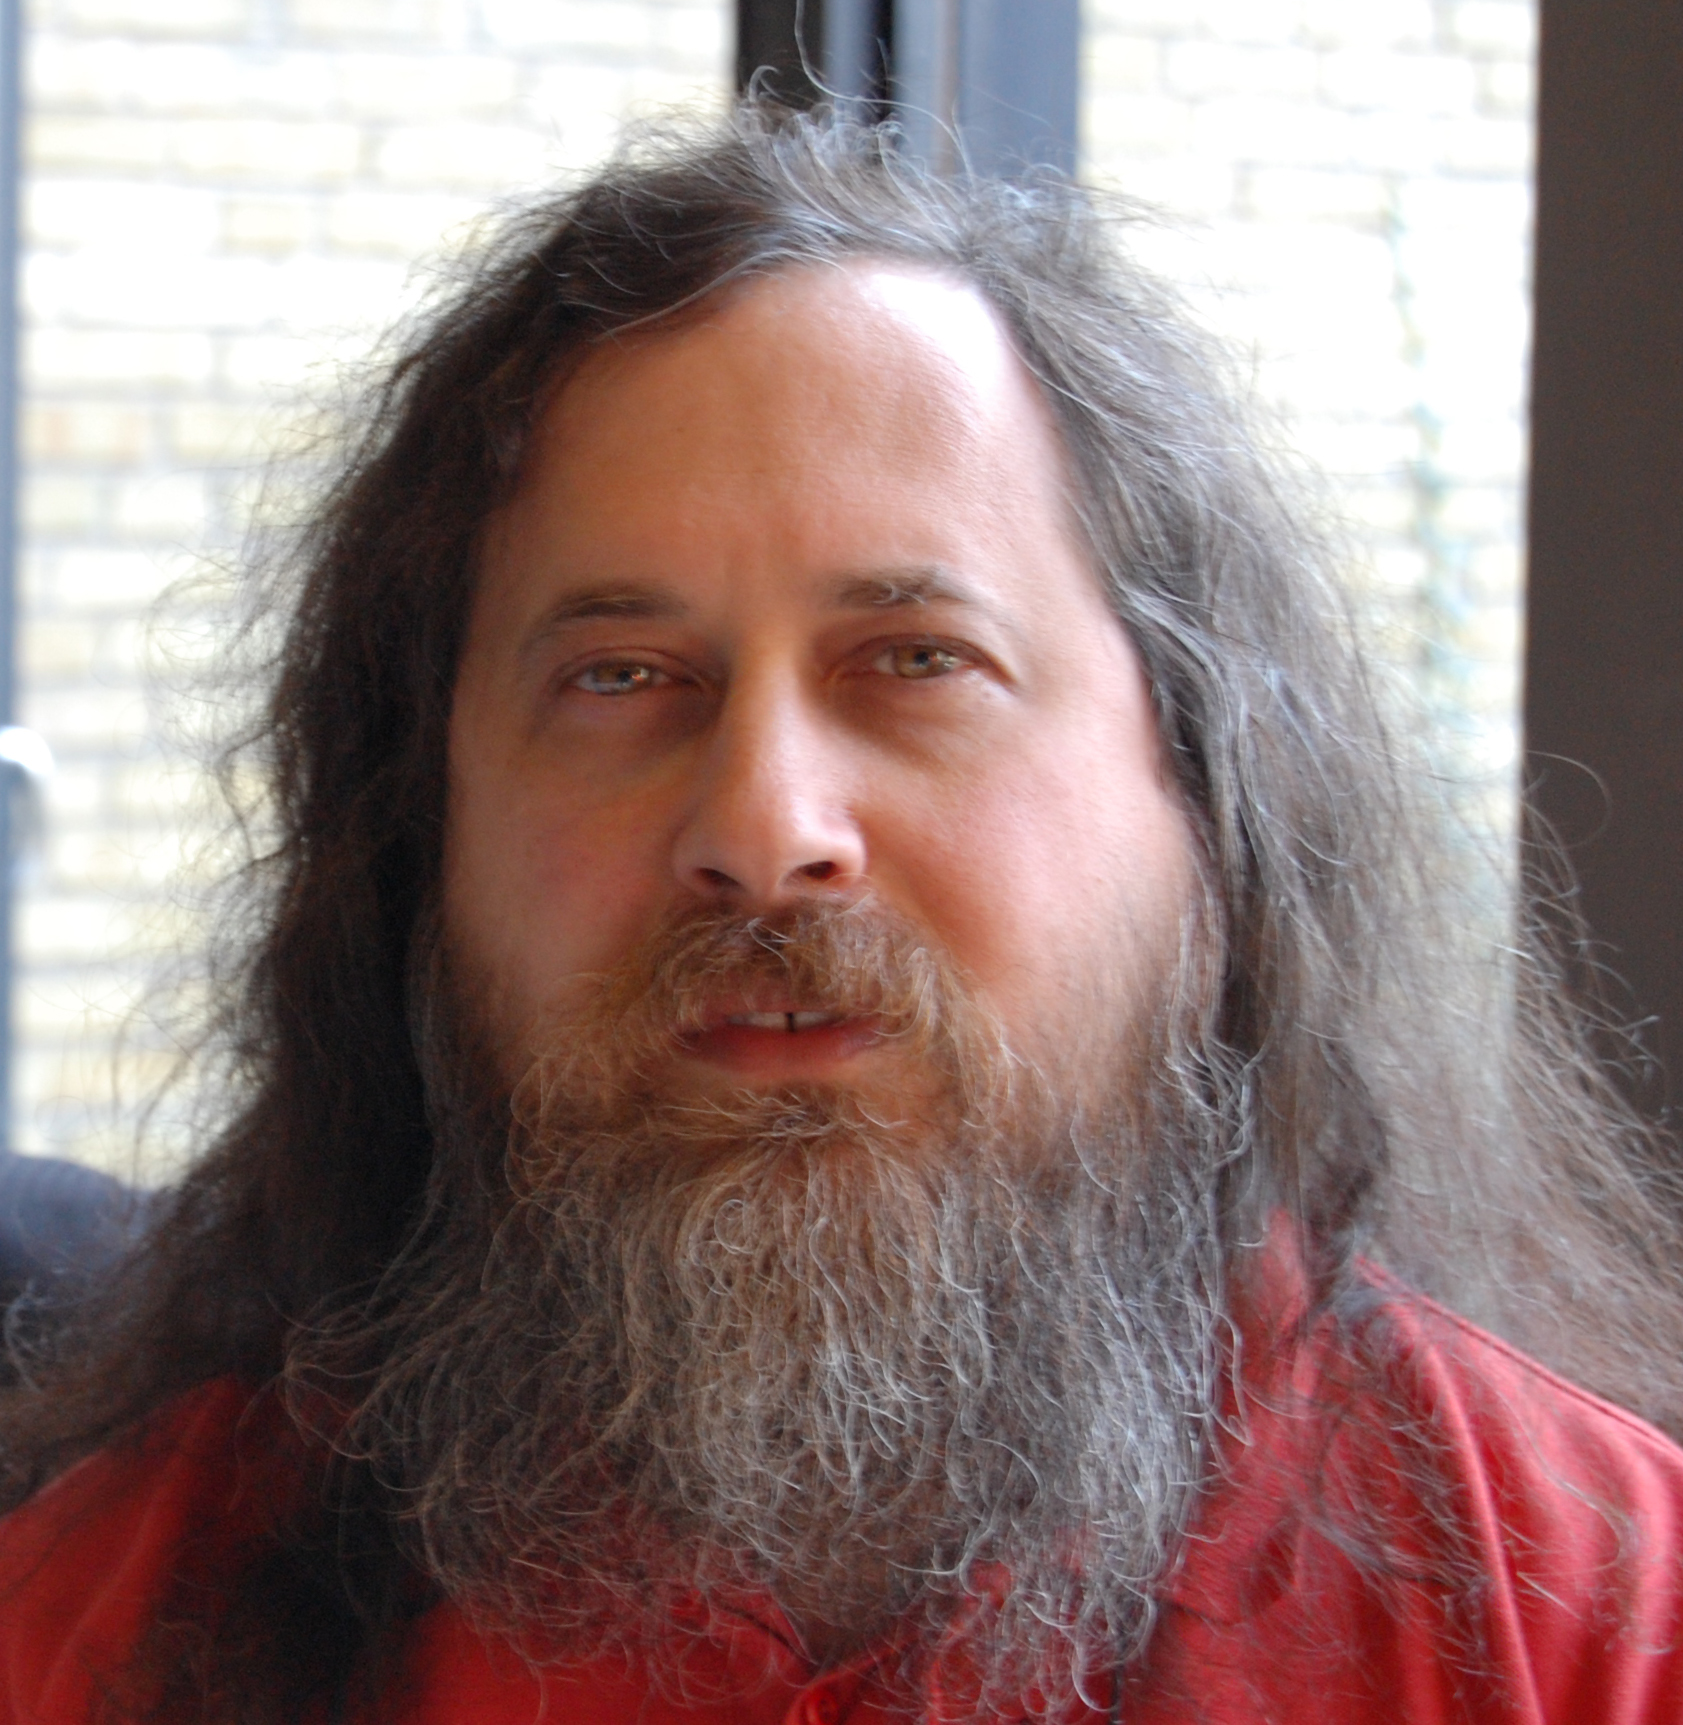
\includegraphics[height=10em]{rms.jpg} 
      &
      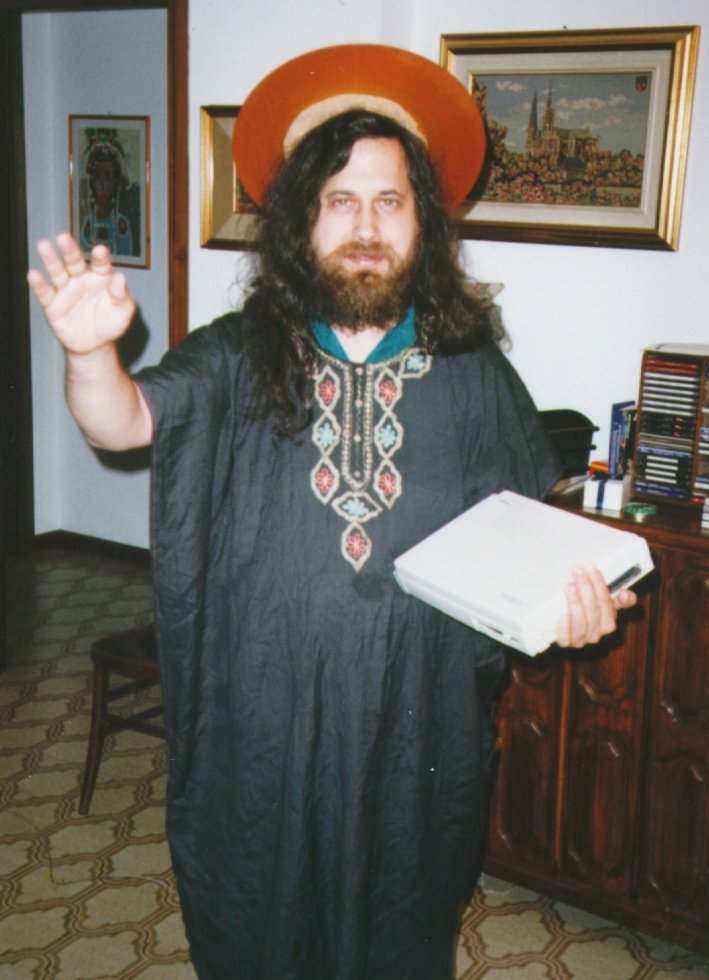
\includegraphics[height=10em]{saintignucius.jpg}
      &
      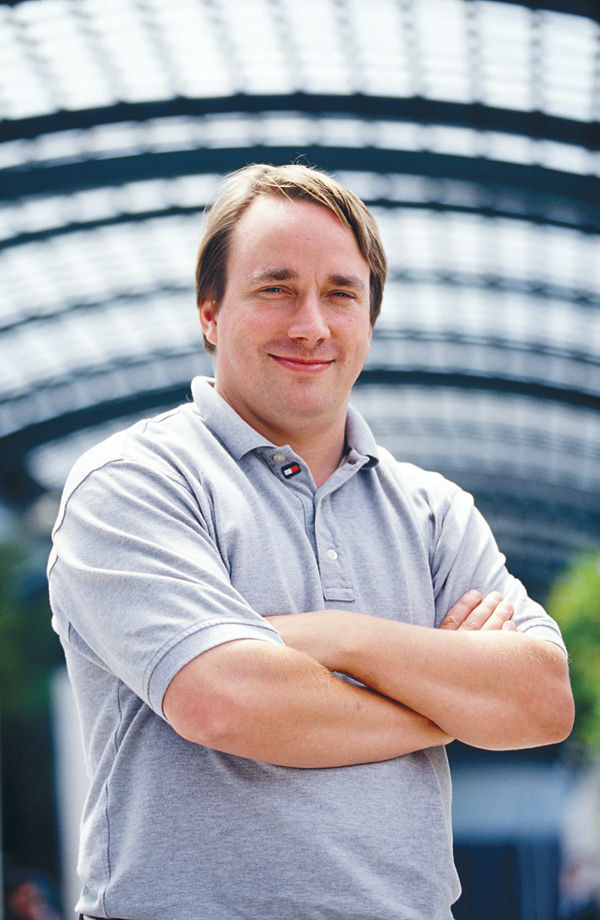
\includegraphics[height=10em]{linus.jpg} 
      & 
      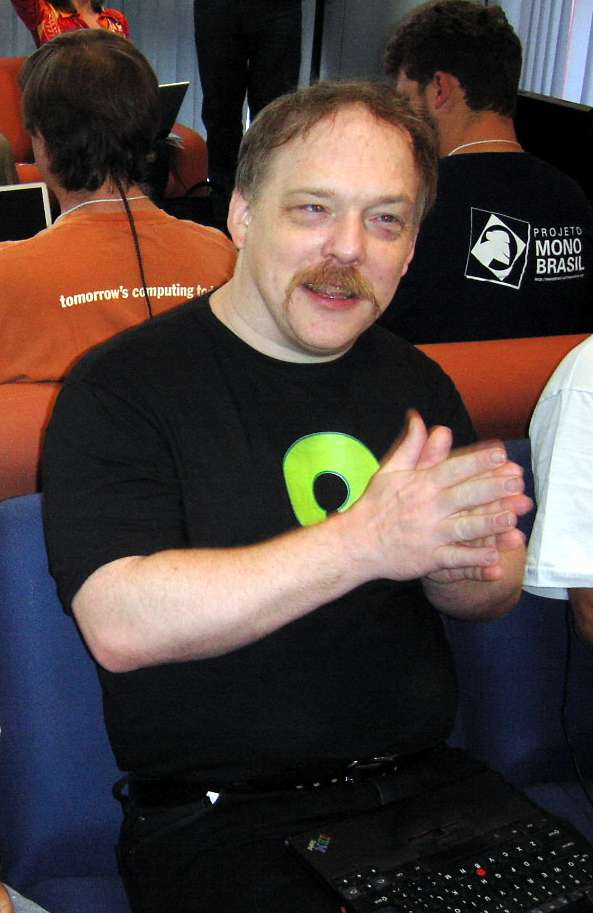
\includegraphics[height=10em]{esr.jpg} 
      \\
      \multicolumn{2}{c}{Richard Stallman}
      &
      Linus Torvalds
      &
      Eric Raymond\\
  \end{tabular}
\end{frame}

%%%%%%%%%%%%%%%%%%%%%%%%%%%%%%%%%%%%%%%%%%%%%%%%%%%%%%%%%%%%%%%%%%%%%%%%%%%%%%

\begin{frame}
  \frametitle{Crédits}

  \small

  \begin{itemize}
  \item Pour cette présentation, je me suis un peu inspiré des cours de
    présentation du logiciel libre que j'ai demandé d'effectuer à certains
    apprentis enseignant-chercheur, qui ont été sous ma responsabilité.

    Ces présentations ont été faites lors du dernier cours magistral de mon
    enseignement de systèmes d'exploitation en DUT informatique.

    Il s'agit des présentations d'Alexis MULLER (en 2004/2005) et Maxime
    MORGE (en 2005/2006).
  
    \vfill
    
  \item Cette présentation et son code source sont mises à disposition
    selon les termes de la
    \href{https://creativecommons.org/licenses/by-nc-sa/3.0/fr/legalcode}{Licence
      Creative Commons Attribution - Pas d’Utilisation Commerciale - Partage
      dans les Mêmes Conditions 3.0 France} \ccbyncsa.

    \vfill

  \item La présentation au format PDF est disponible à \url{http://bruno.boulgour.com/talks/2014/20140204-libre}

    \vfill

  \item Le code source LaTeX de la présentation est disponible à \url{https://github.com/b3/talks-20140204-libre}

  \item La dernière modification de ce document a eu lieu le 05 février 2014 à 17:18 %TS
  \end{itemize}
\end{frame}

\end{document}

% Local Variables:
% time-stamp-line-limit:-20
% time-stamp-start: "le "
% time-stamp-end: " %TS"
% time-stamp-format: "%02d %:b %:y à %:H:%:M"
% time-stamp-active: t
% End:
